\documentclass[compress]{beamer}
\usecolortheme{default}

\usepackage{lmodern, epstopdf, multirow, array, setspace, bbm, tcolorbox, pbox, bm, mathtools, tikz}
\usepackage[T1]{fontenc}

\setbeamertemplate{frametitle}[default][center]
\setbeamertemplate{footline}{\hfill \insertframenumber/\inserttotalframenumber\hspace*{5pt}\vspace{5pt}}
\setbeamertemplate{navigation symbols}{}

\newlength{\wideitemsep}
\setlength{\wideitemsep}{\itemsep}
\addtolength{\wideitemsep}{4pt}
\let\olditem\item
\renewcommand{\item}{\setlength{\itemsep}{\wideitemsep}\olditem}
\setlength{\leftmargini}{12pt}
\setlength{\leftmarginii}{14pt}
\setbeamertemplate{itemize/enumerate subbody begin}{\vspace{6pt}}
\setbeamertemplate{itemize item}[circle]
\setbeamertemplate{enumerate item}[circle]
\setbeamertemplate{enumerate subitem}[default]

\setbeamercolor{alerted text}{fg=blue}
\setbeamersize{text margin left=1.5em,text margin right=1.5em}

\tcbset{
    colback=white,
    colframe=black,
    coltext=black,
    coltitle=blue,
    colbacktitle=white,
    boxrule=1pt,
    titlerule=0pt,
    toptitle=4pt,
    top=2pt
}

\newenvironment{changemargin}[2]{% 
  \begin{list}{}{% 
    \setlength{\topsep}{0pt}% 
    \setlength{\leftmargin}{#1}% 
    \setlength{\rightmargin}{#2}% 
    \setlength{\listparindent}{\parindent}% 
    \setlength{\itemindent}{\parindent}% 
    \setlength{\parsep}{\parskip}% 
  }% 
  \item[]}{\end{list}}
  
\newenvironment{defn}{%
  \begin{tcolorbox}[title={Definition}]%
  }{\end{tcolorbox}}
  
\newenvironment{prop}[1]{%
  \begin{tcolorbox}[title={Proposition #1}]%
  }{\end{tcolorbox}}
  
\newcommand{\cit}[1]{{\footnotesize \textcolor[rgb]{0.5,0,0}{#1}}}

% Font size for code listings (verbatim blocks); reset with \normalsize
\newcommand{\codesize}{\fontsize{7}{8.5}\selectfont}

\newcommand{\slidesetup}[1]{%
  \title{#1}%
  \subtitle{\texorpdfstring{\vspace{0.3\baselineskip}}{} {\small This version: \today}}%
  \author[Mikkel Plagborg-Moller]{ECMA 31150, Spring 2026 \texorpdfstring{\\[0.5ex]}{} University of Chicago \texorpdfstring{\\[0.5ex]}{} Department of Economics \texorpdfstring{\\[4ex]}{} Mikkel Plagborg-Moller}%
  \date{}%
}

% \circleoverlay[options]{text}
% Draws a red circle with a text box nearby on a tikz overlay.
% Options (with defaults):
%   cx=0cm, cy=0cm      - circle center (shift from page center)
%   r=1cm               - circle radius
%   tx=0cm, ty=0cm      - text box offset from circle center
%   text anchor=east    - anchor of text node (east = text left, west = text right)
%   font=\normalsize    - font size for text
\pgfkeys{
  /circleoverlay/.cd,
  cx/.store in=\cocx, cx=0cm,
  cy/.store in=\cocy, cy=0cm,
  r/.store in=\cor, r=1cm,
  tx/.store in=\cotx, tx=0cm,
  ty/.store in=\coty, ty=0cm,
  text anchor/.store in=\cotextanchor, text anchor=east,
  font/.store in=\cofont, font=\normalsize,
}
\newcommand{\circleoverlay}[2][]{%
  \pgfkeys{/circleoverlay/.cd, cx=0cm, cy=0cm, r=1cm, tx=0cm, ty=0cm, text anchor=east, font=\normalsize, #1}%
  \pgfmathsetlengthmacro{\circlediameter}{2*\cor}%
  \node[draw=red, line width=2pt, circle, minimum size=\circlediameter, inner sep=0pt]
    (tmpcirc) at ([xshift=\cocx,yshift=\cocy]current page.center) {};%
  \node[anchor=\cotextanchor, fill=white, draw=red, text=red, inner sep=4pt, align=left, font=\cofont]
    at ([xshift=\cotx,yshift=\coty]tmpcirc.center) {#2};%
}

\DeclareMathOperator*{\argmax}{argmax}
\DeclareMathOperator*{\argmin}{argmin}
\DeclareMathOperator{\diag}{diag}
\DeclareMathOperator{\var}{Var}
\DeclareMathOperator{\cov}{Cov}
\DeclareMathOperator{\corr}{Corr}
\DeclareMathOperator{\lrv}{LRV}


\slidesetup{Forecasting with stationary models II}

\begin{document}
\frame{
\maketitle
}

\frame{
\frametitle{Plan for this slide deck}
\begin{enumerate}
\item Autoregressive (AR) models
\item Estimating/testing AR parameters
\item Selecting the number of lags
\end{enumerate}
}

\frame{
\frametitle{AR(1) model}
\begin{itemize}
\item Let's return to the autoregressive model we saw in the last slide deck:
\begin{equation} \label{eqn:ar1}
y_t = c + \rho y_{t-1} + u_t, \tag{$\dagger$}
\end{equation}
where $c$ and $\rho$ are constants.
\item Assume $u_t$ is white noise satisfying
\[E[u_t \mid y_{t-1},y_{t-2},\dots] = 0.\]
We call $u_t$ the ``shock'' or \textbf{innovation} -- the unforecastable part of $y_t$.
\begin{itemize}
\item In many cases, we'll assume the stronger condition that $u_t$ is i.i.d.\ with mean zero.
\end{itemize}
\item This model is an autoregression of \textbf{order} 1 (one lag): AR(1).
\item When can we find a covariance stationary solution to the stochastic difference equation (\ref{eqn:ar1})?
\end{itemize}
}

\frame{
\frametitle{AR(1) model: stationarity}
\begin{itemize}
\item Since $u_t$ and $y_{t-1}$ are uncorrelated (\alert{why?}),
\[\var(y_t) = \var(c + \rho y_{t-1} + u_t) = \rho^2 \var(y_{t-1}) + \var(u_t).\]
\item If $\lbrace y_t \rbrace$ is covariance stationary, then
\[\var(y_t) = \rho^2 \var(y_t) + \var(u_t) \quad \Longrightarrow \quad \boxed{\var(y_t) = \frac{\sigma_u^2}{1-\rho^2}},\]
where $\sigma_u^2 \equiv \var(u_t)$.
\item Variances must be positive. So covariance stationarity requires $\boxed{-1 < \rho < 1}$.
\end{itemize}
}

\frame{
\begin{figure}
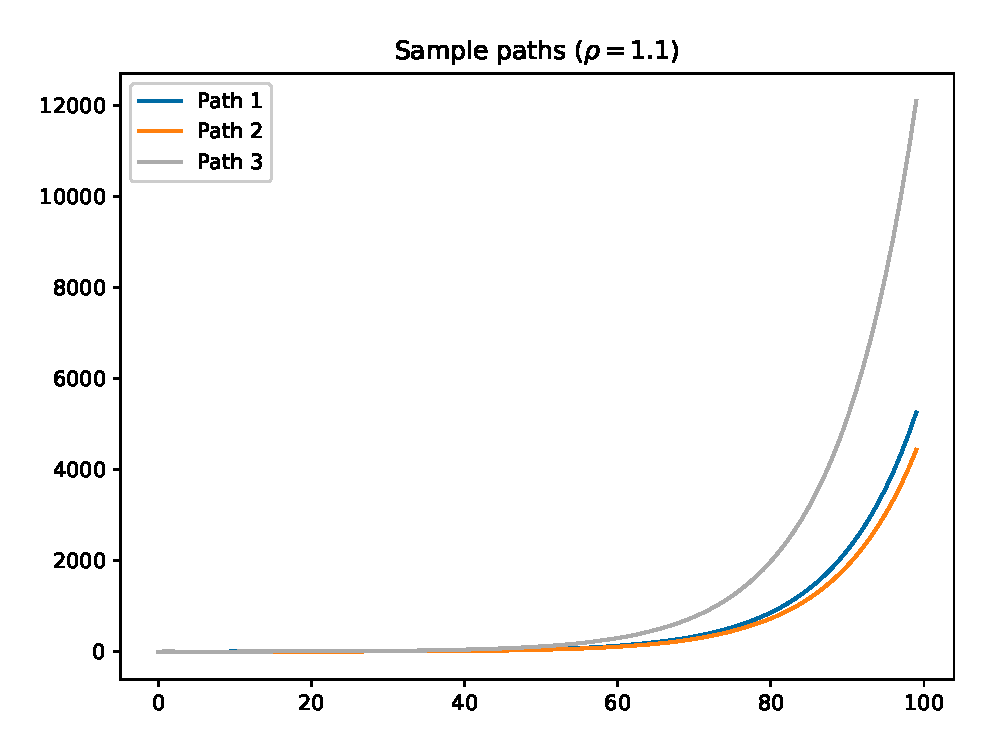
\includegraphics[width=0.8\linewidth]{fig/ar_sim_110.eps} \\
$y_t = \rho y_{t-1} + u_t$, $u_t \overset{iid}{\sim} N(0,1)$, $\rho = 1.1$ \\
\medskip
Explosive behavior $\Rightarrow$ $\var(y_t)$ higher at end of sample $\Rightarrow$ non-stationary
\end{figure}
}

\frame{
\begin{figure}
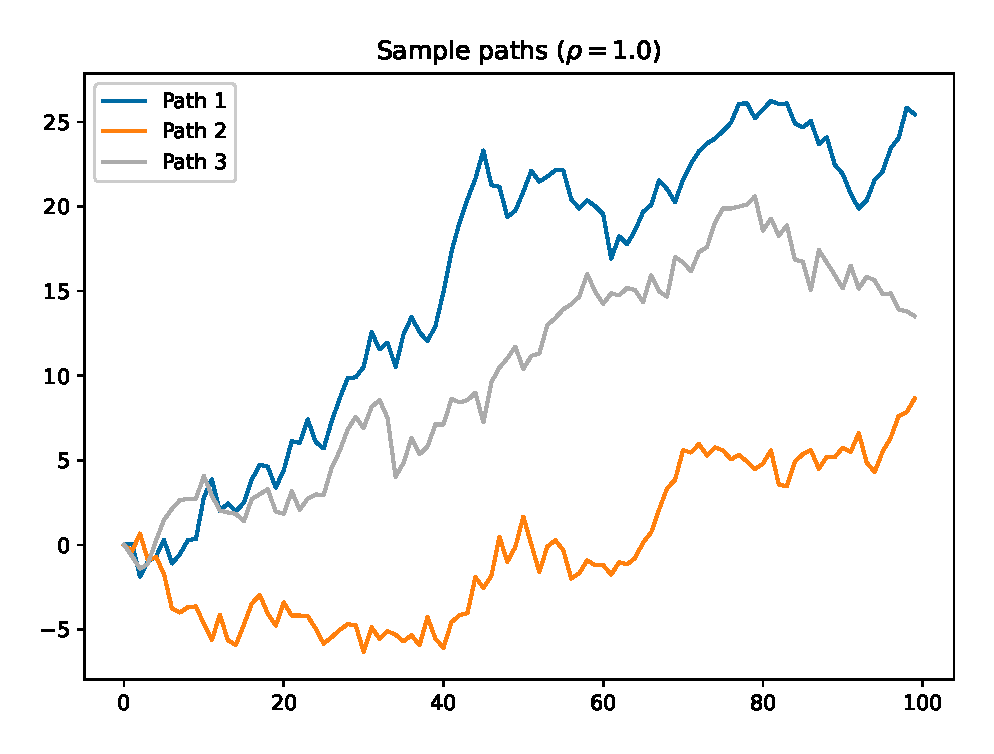
\includegraphics[width=0.8\linewidth]{fig/ar_sim_100.eps} \\
$y_t = \rho y_{t-1} + u_t$, $u_t \overset{iid}{\sim} N(0,1)$, $\rho = 1$ \\
\medskip
Random walk $\Rightarrow$ doesn't mean-revert $\Rightarrow$ non-stationary
\end{figure}
}

\frame{
\begin{figure}
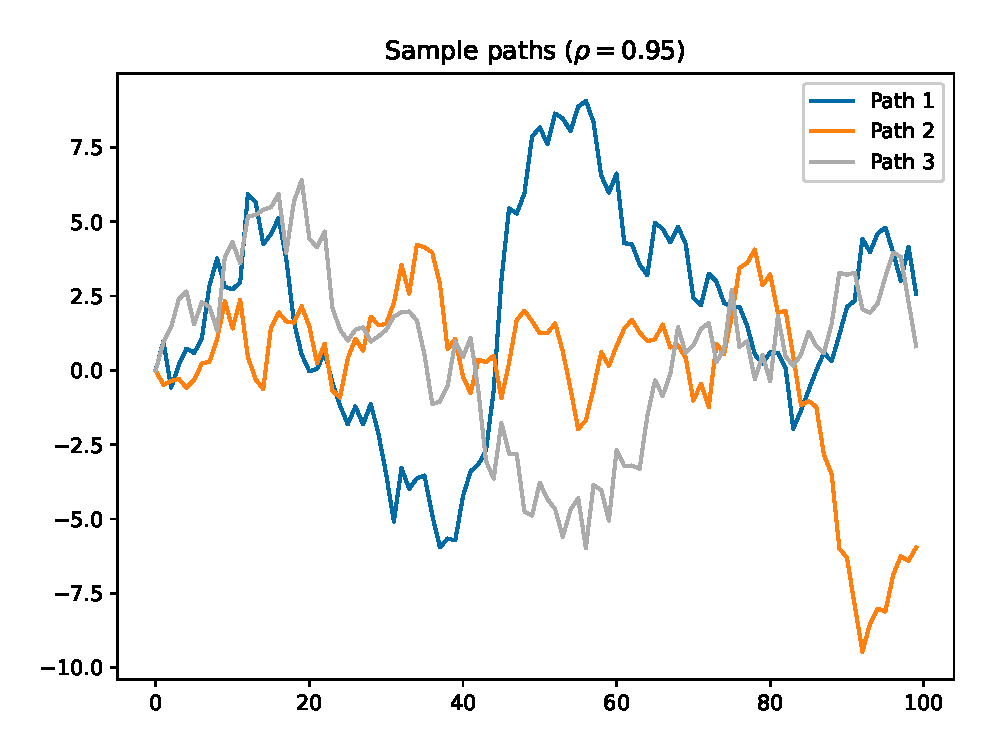
\includegraphics[width=0.8\linewidth]{fig/ar_sim_95.eps} \\
$y_t = \rho y_{t-1} + u_t$, $u_t \overset{iid}{\sim} N(0,1)$, $|\rho|<1$ \\
\medskip
Persistent cycles, but ultimately reverts to mean
\end{figure}
}

\frame{
\frametitle{AR(1): mean and ACF}
\begin{itemize}
\item We derived
\[\var(y_t) = \frac{\sigma_u^2}{1-\rho^2}\]
for a covariance stationary AR(1) process with $-1<\rho<1$.
\item Similar calculations show (\alert{exercise}: verify)
\[\boxed{E(y_t) = \frac{c}{1-\rho}},\quad \boxed{\rho(\ell) \equiv \corr(y_t,y_{t-\ell}) = \rho^\ell},\]
under stationarity.
\end{itemize}
}

\frame{
\frametitle{AR(1): initial condition}
\begin{itemize}
\item For the AR(1) process to be covariance stationary, we also need the \textbf{initial condition} $y_0$ to have these moments:
\[E(y_0) = \frac{c}{1-\rho},\quad \var(y_0) = \frac{\sigma_u^2}{1-\rho^2}.\]
\item Then the previous calculations imply that $y_t$ is covariance stationary.
\begin{itemize}
\item If $u_t \overset{iid}{\sim} N(0,\sigma_u^2)$ and $y_0 \sim N\left(\frac{c}{1-\rho},\frac{\sigma_u^2}{1-\rho^2}\right)$ (independently of the $u_t$'s), then the AR(1) process $\lbrace y_t \rbrace_{t=0}^\infty$ is also strictly stationary.
\end{itemize}
\item If $y_0$ has some other moments, then $\lbrace y_t \rbrace$ will not be covariance stationary, but still,
\[\lim_{t \to \infty} E(y_t) =  \frac{c}{1-\rho},\quad \lim_{t\to\infty}\var(y_t) = \frac{\sigma_u^2}{1-\rho^2},\]
provided $-1<\rho<1$.
\end{itemize}
}

\frame{
\frametitle{AR(1): forecasting}
\[y_t = c + \rho y_{t-1} + u_t\]
\vspace{-0.5\baselineskip}
\begin{itemize}
\item Best guess of next-period observation, given past:
\[E[y_{t+1} \mid y_t,y_{t-1},\dots,y_1] = E[y_{t+1} \mid y_t] = c + \rho y_t + \underbrace{E[u_{t+1} \mid y_t]}_{=0}.\]
\item Best \textbf{one-step-ahead} forecast: $\boxed{y_{t+1|t} \equiv c+\rho y_t}$.
\item In practice, we need to estimate $c$ and $\rho$ to form a feasible forecast (more soon).
\end{itemize}
}

\frame{
\frametitle{AR(1): multi-step forecast}
\begin{itemize}
\item By iterating on the AR(1) equation:
\begin{align*}
y_t &= c + \rho [c + \rho y_{t-2} + u_{t-1}] + u_t \\
&= c + \rho [c + \rho (c + \rho y_{t-3} + u_{t-2}) + u_{t-1}] + u_t \\
&= \dots \\
&= \rho^h y_{t-h} + \sum_{\ell=0}^{h-1} \rho^\ell (c + u_{t-\ell}).
\end{align*}
\item Best \textbf{$h$-step-ahead} forecast:
\[\boxed{y_{t+h|t} \equiv E[y_{t+h} \mid y_t] = \rho^h y_t + \frac{1-\rho^h}{1-\rho}c.}\]
\end{itemize}
}

\frame{
\frametitle{AR($p$) model}
\begin{itemize}
\item Autoregression with $p$ lags, \textbf{AR($p$)}:
\[y_t = c + a_1 y_{t-1} + a_2 y_{t-2} + \dots + a_p y_{t-p} + u_t,\quad E[u_t \mid \lbrace y_s \rbrace_{s<t}]=0.\]
$p+2$ parameters: $c$, $a_1,a_2,\dots,a_p$, and $\sigma_u^2$.
\item If covariance stationary (\alert{verify}):
\[\boxed{E(y_t) = \frac{c}{1-(a_1+a_2+\dots+a_p)}}.\]
\item What is the autocovariance function $\gamma(\ell) \equiv \cov(y_t,y_{t-\ell})$?
\item (Note: We will postpone until a later slide deck the question of when $\lbrace y_t \rbrace$ is actually covariance stationary.)
\end{itemize}
}

\frame{
\frametitle{AR($p$): ACF}
\[y_t = c + a_1 y_{t-1} + a_2 y_{t-2} + \dots + a_p y_{t-p} + u_t,\quad E[u_t \mid \lbrace y_s \rbrace_{s<t}]=0\]
\vspace{-0.5\baselineskip}
\begin{itemize}
\item Assuming covariance stationarity, if we take covariance with respect to $y_{t-\ell}$ on both sides of the above equation, we get
\begin{equation} \label{eqn:ar_acf}
\boxed{\gamma(\ell) = \sum_{j=1}^p a_j \gamma(\ell-j) + \mathbbm{1}(\ell=0)\sigma_u^2}. \tag{$\star$}
\end{equation}
\item If we stack these equations for $\ell=0,1,\dots,p$, we get a system of $p+1$ linear equations (the \textbf{Yule-Walker equations}) in $p+1$ unknowns: $\gamma(0),\gamma(1),\dots,\gamma(p)$.
\begin{itemize}
\item Allows us to solve for the unknowns given the parameters $a_1,\dots,a_p,\sigma_u^2$.
\end{itemize}
\item We can then compute $\gamma(\ell)$ for $\ell > p$ by iterating on (\ref{eqn:ar_acf}).
\begin{itemize}
\item We will soon learn a simpler computational method.
\end{itemize}
\end{itemize}
}

\frame{
\frametitle{Estimation}
\[y_t = c + a_1 y_{t-1} + a_2 y_{t-2} + \dots + a_p y_{t-p} + u_t,\quad E[u_t \mid \lbrace y_s \rbrace_{s<t}]=0\]
\begin{itemize}
\item Given data $y_1,\dots,y_T$, we can estimate $c,a_1,\dots,a_p$ by linear regression (OLS):
\[y_t = \hat{c} + \hat{a}_1 y_{t-1} + \hat{a}_2 y_{t-2} + \dots + \hat{a}_p y_{t-p} + \hat{u}_t.\]
\item The $p$ lags are simply $p$ covariates, as in any other linear regression.
\item $\hat{\sigma}_u^2 \equiv \frac{1}{(T-p)-(p+1)}\sum_{t=p+1}^T \hat{u}_t^2$.
\item Due to the lags, the regression sample starts at $t=p+1$. The effective sample size for the regression is $T-p$, not $T$.
\end{itemize}
}

\frame{
\begin{figure}
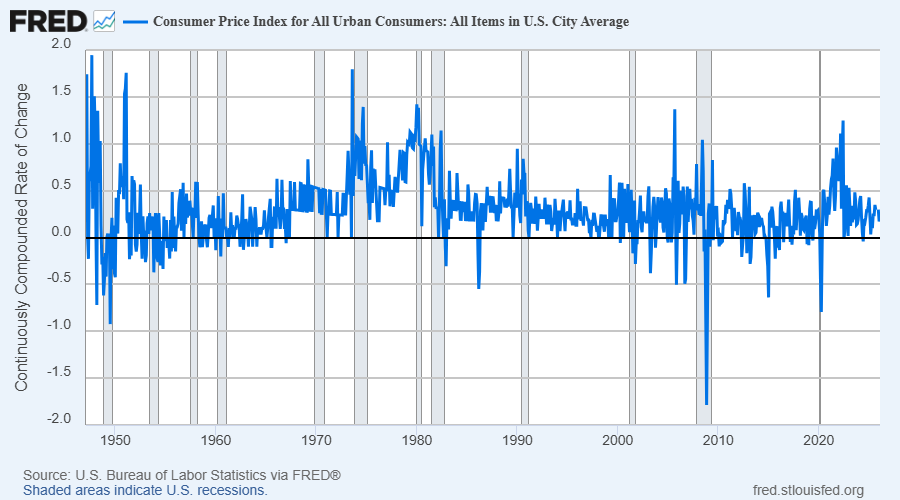
\includegraphics[width=0.9\linewidth]{fig/fred_cpiinfl.png}
\end{figure}
}

\begin{frame}[fragile]
\scriptsize
\begin{verbatim}
import numpy as np
import pandas as pd
import statsmodels.api as sm

# Load data
df = pd.read_csv('data/CPIAUCSL.csv', index_col='observation_date',
    parse_dates=True)
df = df.interpolate() # interpolate missing value in Oct 2025
cpi = df['CPIAUCSL'].values
y = 100*np.diff(np.log(cpi)) # monthly inflation rate

# AR order
p = 3

# Build regressor matrix: columns are lags of y
X = np.column_stack([y[p-j:-j] for j in range(1, p + 1)])
X = sm.add_constant(X)
Y = y[p:]

# OLS estimation
res = sm.OLS(Y, X).fit(cov_type='HC1')
xnames = ['const'] + [f'lag{j}' for j in range(1, p + 1)]
print(res.summary(xname=xnames, slim=True))
print(f'\nResidual std dev: {np.sqrt(res.mse_resid):.4f}')
\end{verbatim}
\end{frame}

\begin{frame}[fragile]
\scriptsize
\begin{verbatim}
                            OLS Regression Results                            
==============================================================================
Dep. Variable:                      y   R-squared:                       0.367
Model:                            OLS   Adj. R-squared:                  0.365
No. Observations:                 946   F-statistic:                     69.29
Covariance Type:                  HC1   Prob (F-statistic):           1.71e-40
==============================================================================
                 coef    std err          z      P>|z|      [0.025      0.975]
------------------------------------------------------------------------------
const          0.0888      0.015      5.933      0.000       0.059       0.118
lag1           0.5050      0.055      9.192      0.000       0.397       0.613
lag2           0.0250      0.053      0.476      0.634      -0.078       0.128
lag3           0.1584      0.046      3.428      0.001       0.068       0.249
==============================================================================

Notes:
[1] Standard Errors are heteroscedasticity robust (HC1)

Residual std dev: 0.2677
\end{verbatim}
\end{frame}

\frame{
\frametitle{OLS estimator: econometric properties}
\begin{itemize}
\item Is the OLS estimator a good estimator?
\begin{enumerate}
\item Is it consistent?
\item Is it unbiased?
\item What is its variance and its distribution?
\end{enumerate}
\end{itemize}
}

\frame{
\frametitle{Consistency}
\begin{itemize}
\item Question {\#}1: is the estimator \textbf{consistent} as $T \to \infty$?
\item Focus on AR(1) model for now, without intercept (everything generalizes): $y_t = \rho y_{t-1} + u_t$.
\item OLS estimator satisfies
\begin{align*}
\hat{\rho} &\equiv \frac{\sum_{t=2}^T y_t y_{t-1}}{\sum_{t=2}^T y_{t-1}^2} = \frac{\sum_{t=2}^T (\rho y_{t-1} + u_t) y_{t-1}}{\sum_{t=2}^T y_{t-1}^2} \\
&= \rho + \frac{\sum_{t=2}^T u_t y_{t-1}}{\sum_{t=2}^T y_{t-1}^2} = \rho + \frac{\frac{1}{T}\sum_{t=2}^T u_t y_{t-1}}{\frac{1}{T}\sum_{t=2}^T y_{t-1}^2}.
\end{align*}
\item In your first econometrics course with i.i.d.\ data, you proved consistency by applying the Law of Large Numbers (LLN) to the numerator and denominator.
\end{itemize}
}

\frame{
\frametitle{Consistency (cont.)}
\[\hat{\rho} = \rho + \frac{\frac{1}{T}\sum_{t=2}^T u_t y_{t-1}}{\frac{1}{T}\sum_{t=2}^T y_{t-1}^2}\]
\begin{itemize}
\item In the AR(1) model, the data $\lbrace y_t \rbrace$ is not independent over time. So the usual LLN does not apply.
\item As long as the data is stationary ($|\rho|<1$), it turns out that the LLN applies unchanged (proof: pset question):
\[\frac{1}{T}\sum_{t=2}^T u_t y_{t-1} \overset{p}{\to} E[u_t y_{t-1}] = 0 \quad \text{(\alert{why?})},\]
\[\frac{1}{T}\sum_{t=2}^T y_{t-1}^2 \overset{p}{\to} E(y_{t-1}^2).\]
\item By the cts.\ mapping theorem, the estimator is consistent if $|\rho|<1$:
\[\hat{\rho} \overset{p}{\to} \rho\quad \text{ as } \quad T \to \infty.\]
\end{itemize}
}

\frame{
\frametitle{Bias}
\begin{itemize}
\item Question {\#}2: is the OLS estimator \textbf{unbiased} in finite samples?
\begin{itemize}
\item We know from your first econometrics course that it is for i.i.d.\ data, if the error term is mean-independent of the regressors.
\item But that proof does not apply here!
\end{itemize}
\begin{align}
E[\hat{\rho}] &= E[E(\hat{\rho} \mid y_1,y_2,\dots,y_{T-1})] \nonumber \\
&= \rho + E\left[\frac{\frac{1}{T}\sum_{t=2}^T E[u_t \mid y_1,\dots,y_{T-1}] y_{t-1}}{\frac{1}{T}\sum_{t=2}^T y_{t-1}^2}\right]. \label{eqn:expn} \tag{$\S$}
\end{align}
\item The error term is \textbf{predetermined} by assumption:
\[E[u_t \mid y_{t-1},y_{t-2},\dots,y_1] = 0.\]
\item But it's not \textbf{strictly exogenous}:
\[E[u_t \mid y_1,\dots,y_{T-1}] = u_t \neq 0\quad \text{for} \quad t \leq T-1.\]
So the expectation of the fraction in (\ref{eqn:expn}) is generally non-zero.
\end{itemize}
}

\frame{
\frametitle{Bias (cont.)}
\begin{itemize}
\item In fact, the OLS estimator (with an intercept) for the AR(1) model displays a \emph{downward} bias in small samples:
\[E[\hat{\rho}] - \rho \approx -\frac{1+3\rho}{T}.\]
\item The bias vanishes as $T \to \infty$ (after all, $\hat{\rho}$ is consistent).
\item But it can be substantial in small samples, especially when $\rho \approx 1$.
\item In AR($p$) models, OLS is also biased in small samples and tends to indicate that the data is less persistent than it really is.
\end{itemize}
}

\frame{
\frametitle{Asymptotic normality}
\begin{itemize}
\item Question {\#}3: what's the distribution of the OLS estimator?
\item If the data were i.i.d., the Central Limit Theorem (CLT) would tell us
\begin{equation} \label{eqn:clt}
\sqrt{T} \frac{1}{T}\sum_{t=2}^T u_t y_{t-1} \overset{d}{\to} N\left(0,E[u_t^2y_{t-1}^2]\right). \tag{$\sharp$}
\end{equation}
\item But our data is not i.i.d. However, the product $u_t y_{t-1}$ is a MDS:
\[E[u_t y_{t-1} \mid y_{t-1},y_{t-2},\dots] = y_{t-1} \times E[u_t \mid y_{t-1},y_{t-2},\dots] = 0.\]
\item It turns out that the CLT can be generalized to allow for MDS's, so (\ref{eqn:clt}) still applies.
\end{itemize}
}

\frame{
\frametitle{Standard errors and testing}
\begin{itemize}
\item With the CLT in hand, Slutsky's Lemma implies
\[\sqrt{T}(\hat{\rho} - \rho) = \frac{\sqrt{T}\frac{1}{T}\sum_{t=2}^T u_t y_{t-1}}{\frac{1}{T}\sum_{t=2}^T y_{t-1}^2} \overset{d}{\to} \frac{N\left(0,E[u_t^2y_{t-1}^2]\right)}{E(y_{t-1}^2)}.\]
\item Loosely:
\[\boxed{\hat{\rho} \overset{approx}{\sim} N\left(\rho, \frac{1}{T} \times \frac{E[u_t^2y_{t-1}^2]}{\left(E[y_{t-1}^2]\right)^2} \right)}.\]
\item You may not remember, but this is exactly the same variance expression as in the case of i.i.d.\ data -- though the proof is different!
\item Practical upshot: we can use the same formulas for standard errors, t-tests, and F-tests as you learned in your first econometrics course.
\end{itemize}
}

\begin{frame}[fragile]
\scriptsize
\begin{verbatim}
                            OLS Regression Results                            
==============================================================================
Dep. Variable:                      y   R-squared:                       0.367
Model:                            OLS   Adj. R-squared:                  0.365
No. Observations:                 946   F-statistic:                     69.29
Covariance Type:                  HC1   Prob (F-statistic):           1.71e-40
==============================================================================
                 coef    std err          z      P>|z|      [0.025      0.975]
------------------------------------------------------------------------------
const          0.0888      0.015      5.933      0.000       0.059       0.118
lag1           0.5050      0.055      9.192      0.000       0.397       0.613
lag2           0.0250      0.053      0.476      0.634      -0.078       0.128
lag3           0.1584      0.046      3.428      0.001       0.068       0.249
==============================================================================

Notes:
[1] Standard Errors are heteroscedasticity robust (HC1)
\end{verbatim}

\bigskip
\normalsize
\begin{itemize}
\item 95\% confidence interval for $a_1$: $[0.397, 0.613]$
\item Coefficient on 2nd lag is insignificant at 10\% level.
\item F-test rejects that process is white noise w.\ p-value $<2 \times 10^{-40}$.
\end{itemize}
\end{frame}

\begin{frame}[fragile]
\frametitle{Simulation illustration of econometric properties}
\footnotesize
\begin{verbatim}
# Parameters
rho = 0.9
T = 100
n_sim = 5000
rng = np.random.default_rng(seed=31150)

# Monte Carlo loop
rho_hat = np.zeros(n_sim)
for i in range(n_sim):
    # Simulate AR(1)
    u = rng.standard_normal(T)
    y = np.zeros(T)
    for t in range(1, T):
        y[t] = rho * y[t - 1] + u[t]
    # OLS estimation
    X = sm.add_constant(y[:-1])
    Y = y[1:]
    res = sm.OLS(Y, X).fit()
    rho_hat[i] = res.params[1]
\end{verbatim}
\end{frame}

\frame{
\begin{figure}
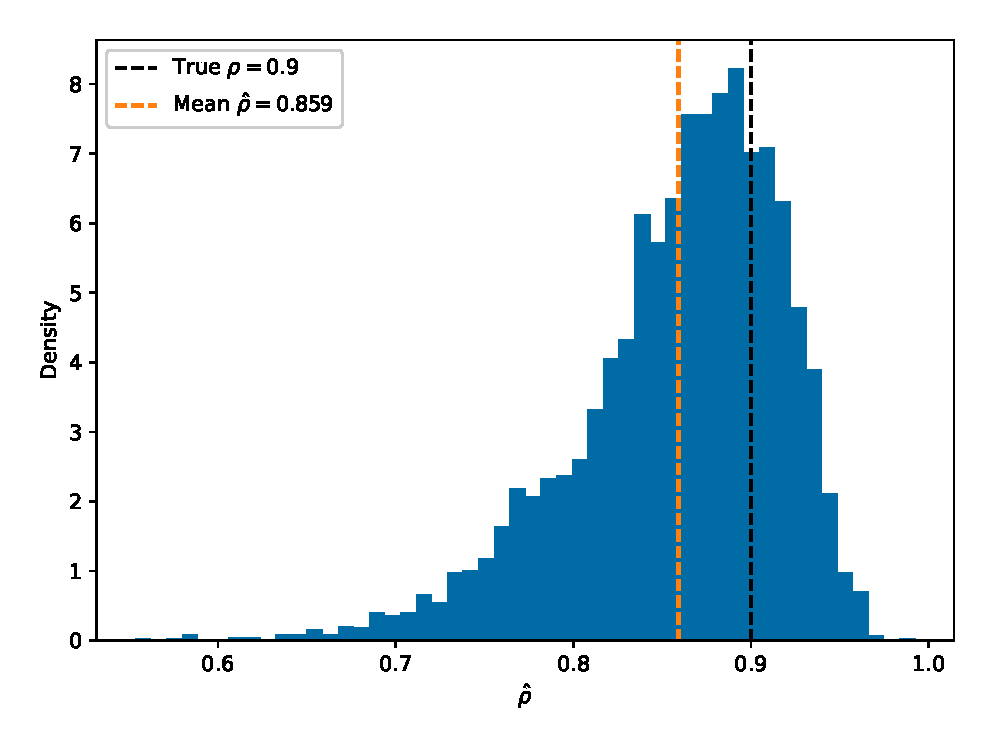
\includegraphics[width=0.9\linewidth]{fig/mc_ar1_T100.eps} \\
$T=100$
\end{figure}
}

\frame{
\begin{figure}
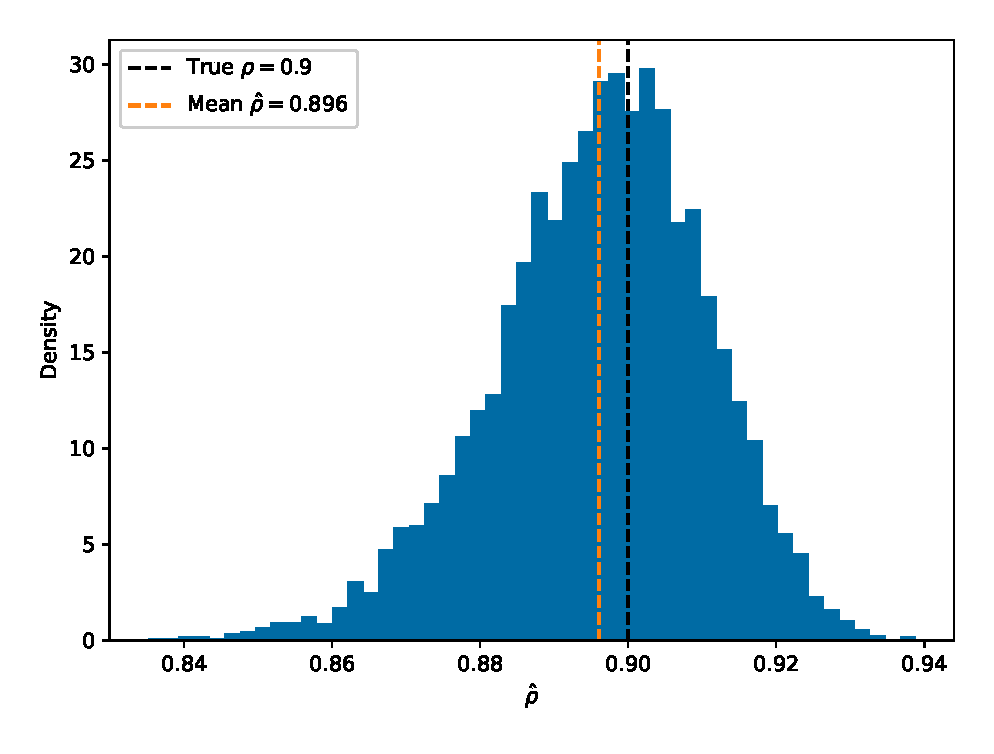
\includegraphics[width=0.9\linewidth]{fig/mc_ar1_T1000.eps} \\
$T=1000$ (notice different horizontal axis limits)
\end{figure}
}

\frame{
\frametitle{Lag order selection}
\begin{itemize}
\item How many lags $p$ to include in our AR($p$) regression?
\item Bias-variance trade-off:
\begin{itemize}
	\item More lags: better fit complicated dynamics $\Rightarrow$ lower bias.
	\item Fewer lags: fewer parameters to estimate $\Rightarrow$ lower variance.
\end{itemize}
\end{itemize}
}

\frame{
\frametitle{Lag order selection: general-to-specific}
\begin{itemize}
\item One strategy for picking $p$: \textbf{general-to-specific testing}.
\begin{enumerate}
\item Start with large $p$.
\item Test whether coefficient on $p$-th lag is zero at signif.\ level $\alpha$.
\item If don't reject, estimate AR($p-1$) model.
\item Test whether the last coefficient is zero.
\item Continue until we reject, then stop.
\end{enumerate}
\item This strategy has probability of at least $\alpha$ (in practice, often much higher) of selecting too large a model, since every test in the sequence may falsely reject (type-I error).
\end{itemize}
}

\frame{
\frametitle{Lag order selection: BIC}
\begin{itemize}
\item Instead, it's common to select $p$ to minimize the \textbf{Bayesian information criterion} (BIC):
\[\mathit{BIC}(p) \equiv \log \lbrace \hat{\sigma}(p)^2 \rbrace + p \times \frac{\log T_\text{eff}}{T_\text{eff}}.\]
\vspace{-\baselineskip}
\begin{itemize}
\item $\hat{\sigma}(p)^2 \equiv $ sample variance of OLS residuals from AR($p$) regression.
\item $T_\text{eff} \equiv $ effective sample size (\# obs.\ in the regression).
\end{itemize}
\item This criterion intuitively captures the bias-variance trade-off:
\begin{itemize}
\item Larger $p$ improves fit so decreases first term.
\item Second term penalizes complex models with large $p$.
\end{itemize}
\item The BIC is \textbf{consistent}: if data is generated by an AR($p_0$), then
\[\textstyle P\left(p_0 \in \argmin_p \mathit{BIC}(p)\right) \to 1 \quad \text{as} \quad T\to\infty.\]
\end{itemize}
}

\frame{
\frametitle{Lag order selection: AIC}
\begin{itemize}
\item A variant of the BIC is the \textbf{Akaike information criterion} (AIC):
\[\mathit{AIC}(p) \equiv \log \lbrace \hat{\sigma}(p)^2 \rbrace + p \times \frac{2}{T_\text{eff}}.\]
\item When $T_\text{eff} \geq 8$ (so $\log(T_\text{eff}) > 2$), AIC penalizes complex models less than BIC, so selects (weakly) larger models.
\item As a result, AIC is \emph{inconsistent}: positive probability of selecting too large models, even when $T$ is very large.
\item However, AR forecasts made with $p$ selected by AIC are \textbf{efficient}: when the true model has $\infty$-ly many lags, the forecast errors tend to be smaller on average than those made with any other lag order selection method, at least when $T$ is large.
\item Dilemma: consistency or efficiency? Since AR models are at best approximations, efficiency seems more relevant.
\end{itemize}
}

\begin{frame}[fragile]
\scriptsize
\begin{verbatim}
p_max = 24 # max lag order
p_grid = np.arange(1, p_max + 1)
Y = y[p_max:]
T_eff = len(Y)
aic = np.zeros(p_max)
bic = np.zeros(p_max)

for i, p in enumerate(p_grid):
    # Build regressor matrix (enforce same sample for all p)
    X = np.column_stack([y[p_max-j:-j] for j in range(1, p + 1)])
    X = sm.add_constant(X)
    # OLS estimation
    res = sm.OLS(Y, X).fit()
    sigma2 = np.var(res.resid)
    # Information criteria
    aic[i] = np.log(sigma2) + 2 * p / T_eff
    bic[i] = np.log(sigma2) + np.log(T_eff) * p / T_eff
\end{verbatim}
\bigskip
\normalsize
Note: it's conventional to run all AR regressions on the same sample $t=p_{\max}+1,p_{\max}+2,\dots,T$, so $T_\text{eff}=T-p_{\max}$.
\end{frame}

\frame{
\begin{figure}
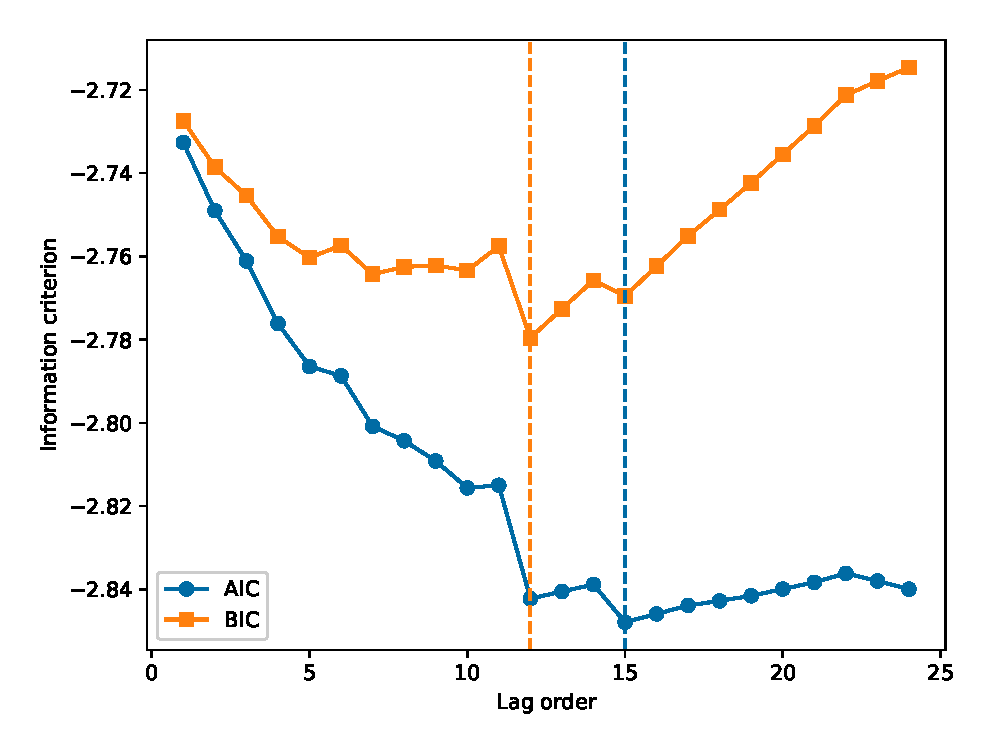
\includegraphics[width=0.9\linewidth]{fig/ic.eps}
\end{figure}
}

\frame{
\frametitle{Practical coding}
\begin{itemize}
\item For pedagogical reasons, my Python code computed AR estimates and information criteria ``by hand'' from OLS output.
\item But in practice, we can use {\tt statsmodels}'s built-in functions for AR modeling:
\begin{itemize}
\item Estimation and inference: \texttt{statsmodels.tsa.ar\_model.AutoReg}
\item BIC/AIC: \texttt{statsmodels.tsa.ar\_model.ar\_select\_order}
\end{itemize}
\end{itemize}
}

\frame{
\frametitle{What did we learn?}
\begin{itemize}
\item AR($p$) model
\begin{itemize}
\item Estimation by OLS
\item Econometric properties: consistency, bias, asymptotic normality
\item Standard errors, testing
\end{itemize}
\item Lag length selection
\begin{itemize}
\item General-to-specific testing
\item BIC, AIC, consistency vs.\ efficiency
\end{itemize}
\end{itemize}
}

\frame{
\frametitle{Looking ahead}
\begin{itemize}
\item What are the sources of forecast errors?
\item How do we evaluate the quality of forecasts?
\item Forecast intervals: conveying uncertainty about forecasts
\end{itemize}
}

\end{document}
